\section{Results}
\label{sec:results}

Figure \ref{fig:dynamics} shows the initial sea surface height (solid black) and compares the adjusted height and velocity profiles between numerical (solid) and analytical (dashed) solutions. Overall, there is good agreement in shape and magnitude. There are small discrepancies close to the boundaries where the numerical solution underestimates sea surface height and meridional velocity.
\begin{figure}[htbp]
	\centering
	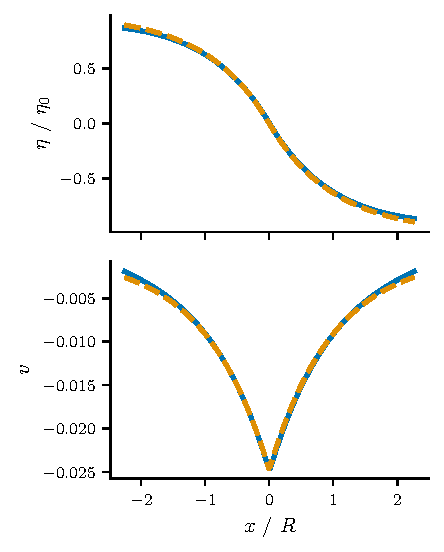
\includegraphics{dynamics_comparison}
	\caption{Upper: relative sea surface height. Lower: meridional velocity. Solid line shows numerical result, while dashed line shows analytical results.}
	\label{fig:dynamics}
\end{figure}

The time evolution of relative potential (blue) and kinetic energy (orange) of the system is shown in Figure \ref{fig:energetics}. The black lines marks a 1/3 and 2/3. We see that $V$ and $K$ fluctuate initially before converging to 2/3 for the potential energy and 1/3 for the kinetic energy, in agreement with theory.
\begin{figure}[htbp]
	\centering
	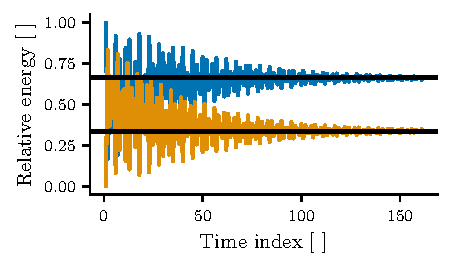
\includegraphics{energetics}
	\caption{Relative energies where blue line shows potential energy and orange line shows kinetic energy. The horizontal black lines marks a 1/3 and 2/3.}
	\label{fig:energetics}
\end{figure}